\documentclass{article}
\usepackage{iclr2026_conference,times}

% =====================================================================
% INTERNAL DRAFT NOTE -- REMOVE BEFORE SUBMISSION
% Numbers explicitly marked \placeholder are SIMULATED PLACEHOLDERS.
% The current-build audit in Table 2 is measured from benchmark_v2.json.
% Replace all simulated results with real evaluation logs before submission.
% =====================================================================

\usepackage{amsmath,amssymb}
\usepackage{booktabs}
\usepackage{graphicx}
\usepackage{multirow}
\usepackage{xcolor}
\usepackage{enumitem}
\usepackage{url}
\usepackage{microtype}
\usepackage[hidelinks]{hyperref}
\usepackage{natbib}

\newcommand{\bench}{\textsc{LiveSearchVQA}}
\newcommand{\acb}{\mathrm{Acc}_{\mathrm{CB}}}
\newcommand{\aws}{\mathrm{Acc}_{\mathrm{WS}}}
\newcommand{\aor}{\mathrm{Acc}_{\mathrm{OR}}}
\newcommand{\placeholder}[1]{\textcolor{blue!65!black}{#1}}
\newcommand{\draftnote}{\textcolor{blue!65!black}{\textit{simulated draft value}}}
\newcounter{algorithm}

\title{\bench: Certifying Search Necessity\\
for Web-Search Agents}

\author{Anonymous Authors\\Affiliation withheld\\\texttt{email withheld}}
\date{}

\begin{document}
\maketitle

\begin{abstract}
Fresh questions alone do not identify whether a vision--language agent knew
an answer, retrieved it, or failed to use evidence already found.
We introduce \bench{}, an on-demand visual question answering benchmark built
from image-bearing English news published within the preceding 48 hours.
Its core output is a \emph{certificate-carrying item}: the image must resolve
the queried event (P0), a heterogeneous panel must fail without web evidence
(P1: empirical search necessity), and every panel member must succeed when
given the gold evidence (P2: evidence sufficiency).
An asymmetric two-module engine constructs this contract.
The \emph{generator} selects verbatim evidence before writing an
event-specific question and performs a same-call closed-book self-check;
the independent, rejection-only \emph{quality module} is the sole admission
authority.
Typed rejection logs improve later explicitly triggered builds, but never
replace certification.
A logically exact cascade reduces verification cost without changing the
admitted set, and every release stores the complete provenance, alignment
audits, and P1/P2 traces.
The resulting closed-book / with-search / oracle protocol separates retrieval
misses, distraction, and evidence-utilization failures.
Our current public build contains 200 validated items from 23 English
sources, of which 78.5\% ask for numeric or temporal facts.
In our planned 12-agent study, the leading system realizes only
\placeholder{74.0\%} of its certified search headroom despite
\placeholder{99.0\%} oracle accuracy, suggesting that retrieval rather than
question answerability is the principal bottleneck.
\end{abstract}

\section{Introduction}
\label{sec:intro}

Modern multimodal assistants identify a pictured entity or event, formulate
web queries, inspect pages, and ground a response in newly published evidence.
A useful benchmark must therefore answer a harder question than whether the
final answer was correct: \emph{where did the search loop fail?}

Static knowledge VQA benchmarks such as OK-VQA, A-OKVQA, and InfoSeek
\citep{okvqa,aokvqa,infoseek} are valuable measures of external knowledge,
but their answers can migrate into model parameters.
Fresh or dynamic benchmarks reduce this risk \citep{freshqa,dynvqa,livebench},
yet freshness alone does not imply search necessity.
A newly published question may ask a stable biographical fact, expose the
answer in the image, or be guessed from its wording.
At the opposite extreme, automatically generated questions may be fresh but
ambiguous, visually unrelated, or unsupported by the cited article.

We address both failure modes by treating automatic construction as a
\emph{generate--verify} contract rather than a loose generation--filtering
sequence.
The two modules have deliberately different responsibilities:
\begin{itemize}[leftmargin=*,itemsep=2pt]
  \item The \textbf{generator module} shapes the proposal distribution toward
  questions likely to satisfy our contract. It starts from an event-specific
  evidence span, constructs an image-dependent question around that span, and
  rejects its own candidate if a closed-book answer is already available.
  \item The \textbf{quality module} never trusts the proposal. It checks
  freshness, exact evidence, image--article alignment, image-dependent
  reference, and finally P1/P2 with a three-model, four-sample panel.
  It returns both an admission decision and a typed audit trail.
\end{itemize}

This asymmetry separates efficiency from validity.
Generation is optimized for proposal recall and cost, whereas verification is
optimized for precision and trust.
The verifier's feedback becomes negative rules and positive exemplars for the
next explicitly triggered build, but it never changes the admission rule.
We therefore do not ask reviewers to trust the generator; trust comes from a
frozen, replayable item contract and its retained audit record.

The resulting item is pinned between two experimentally checked endpoints.
Without evidence, every panel attempt is wrong; with the exact evidence,
every attempt is correct.
An evaluated agent's with-search behavior lies between these endpoints.
If it fails, its retrieval trace lets us distinguish an absent gold fact
(\emph{retrieval miss}), a present but ignored gold fact
(\emph{utilization}), or selection of a competing stale passage
(\emph{distraction}).

Our contributions are:
\begin{enumerate}[leftmargin=*,itemsep=2pt]
  \item an on-demand, open-ended, image-grounded VQA benchmark whose freshness,
  visual dependence, search necessity, and answerability are re-established
  per item rather than inferred from publication time;
  \item a certificate-carrying generator--quality architecture that combines
  evidence-first proposal, same-call self-screening, multimodal alignment,
  and panel-based necessity/sufficiency certification;
  \item a logically exact cascade: closed-book uses OR rejection and oracle
  uses AND admission, enabling early stopping on rejected candidates while
  preserving full evidence for every admitted item;
  \item a three-condition diagnostic protocol and auditable data format that
  attribute search errors to retrieval, distraction, or utilization.
\end{enumerate}

\begin{figure}[t]
  \centering
  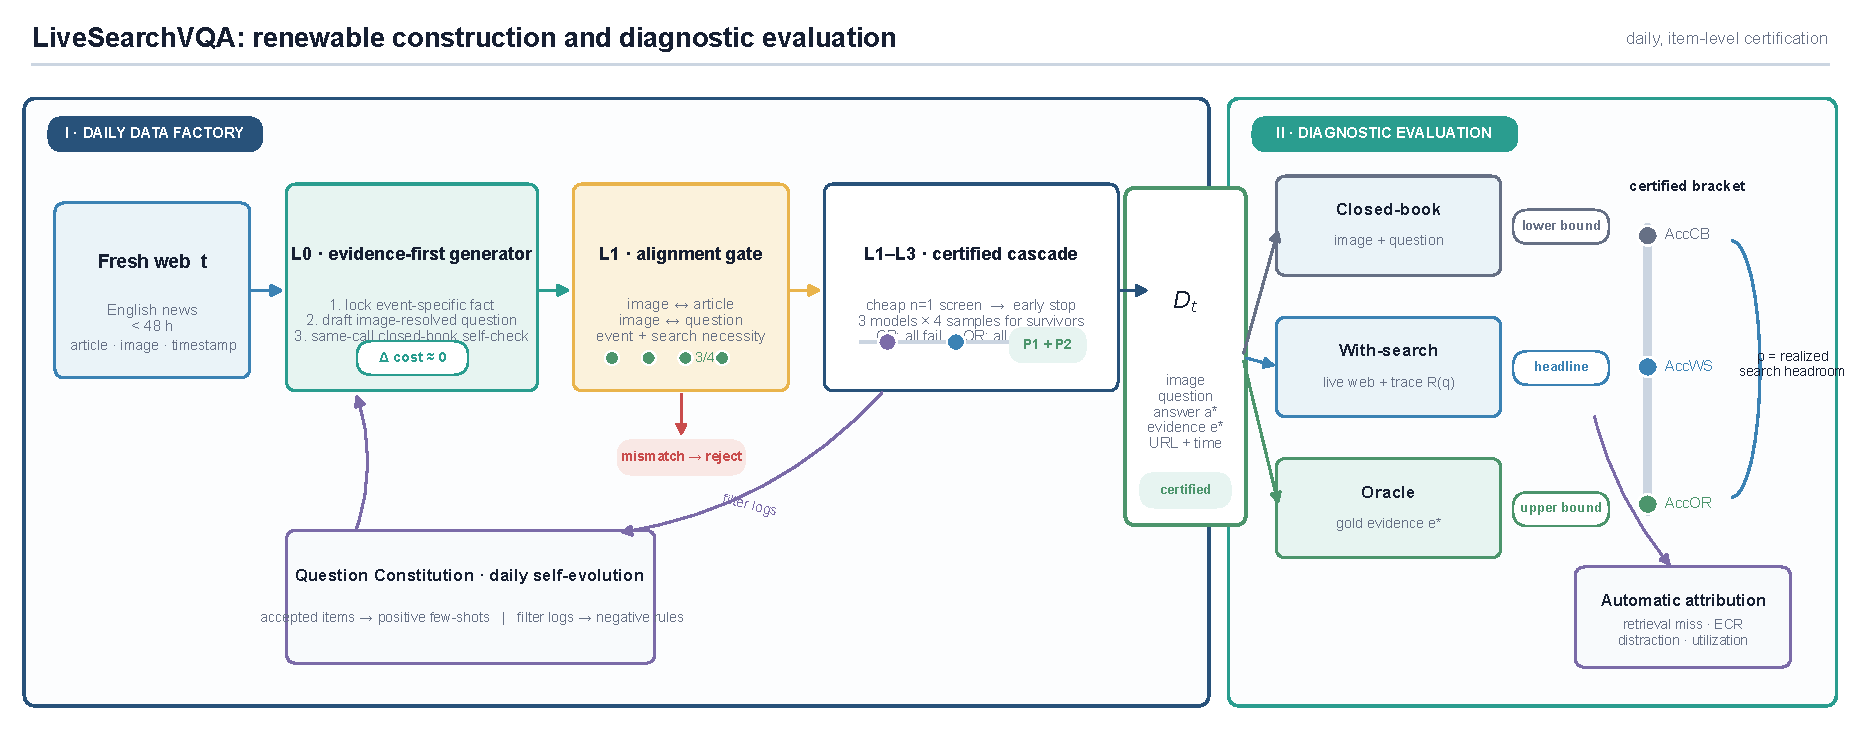
\includegraphics[width=\linewidth]{figures/fig1_system_overview.pdf}
  \caption{\textbf{System overview.} The generator proposes evidence-first,
  image-dependent questions; the quality module certifies visual grounding,
  search necessity (P1), and evidence sufficiency (P2). Accepted items and
  typed rejection logs are both useful outputs: the former forms the released
  benchmark, while the latter improves subsequent explicit builds.}
  \label{fig:overview}
\end{figure}

\section{Related Work}

\paragraph{Knowledge-intensive and visual search benchmarks.}
OK-VQA and A-OKVQA test knowledge beyond pixels, while InfoSeek and MMSearch
more directly study information-seeking VLMs
\citep{okvqa,aokvqa,infoseek,mmsearch}.
These datasets are static and generally do not provide a per-item
counterfactual showing that search is necessary for current models.

\paragraph{Fresh and dynamic evaluation.}
FreshQA, Dyn-VQA, LiveBench, and LiveVQA reduce contamination through recent
or changing content \citep{freshqa,dynvqa,livebench,livevqa}.
\bench{} differs in combining a sub-48-hour collection window with on-demand
re-certification, open-ended visual questions, verbatim evidence, and an
oracle-conditioned sufficiency test.

\paragraph{Browsing agents.}
GAIA and BrowseComp evaluate tool use and hard-to-find factual reasoning
\citep{gaia,browsecomp}.
They emphasize end-task difficulty.
Our emphasis is complementary: a renewable visual stream whose verified
endpoints make error attribution possible.

\begin{table}[t]
\centering
\small
\setlength{\tabcolsep}{4pt}
\begin{tabular}{lccccc}
\toprule
Benchmark & Visual & Refresh & P1 & P2 & Diagnosis\\
\midrule
OK-VQA / A-OKVQA & \checkmark & -- & -- & -- & --\\
InfoSeek / MMSearch & \checkmark & -- & -- & -- & partial\\
FreshQA / LiveBench & -- & periodic & -- & partial & --\\
LiveVQA & \checkmark & snapshot & -- & partial & --\\
\textbf{\bench{}} & \checkmark & \textbf{on demand} & \checkmark & \checkmark & \checkmark\\
\bottomrule
\end{tabular}
\caption{Positioning of \bench{}. P1 denotes verified search necessity and P2
denotes verified answerability from gold evidence.}
\label{tab:related}
\end{table}

\section{The Generate--Verify Data Engine}
\label{sec:method}

\subsection{Item contract}
An item is $x=(I,q,a,e,u,t)$: image $I$, English open-ended question $q$,
short answer $a$, verbatim evidence $e$, source URL $u$, and publication time
$t$.
The quality module admits $x$ only if three properties hold.

\paragraph{P0: multimodal grounding.}
The image and article depict the same event or entity; $I$ resolves an
otherwise omitted referent in $q$; and $a$ is not readable from pixels alone.

\paragraph{P1: empirical search necessity.}
For a panel $\mathcal{M}$ and stochastic runs $r\in\{1,\ldots,R\}$,
\begin{equation}
\forall m\in\mathcal{M},\forall r:\quad
\mathrm{Eq}(m(I,q;r),a)=0.
\label{eq:p1}
\end{equation}
This is a panel-relative empirical certificate, not a universal proof for all
future models. We make that scope explicit and preserve every prediction so
the certificate can be replayed as panels improve.

\paragraph{P2: evidence sufficiency.}
\begin{equation}
\forall m\in\mathcal{M},\forall r:\quad
\mathrm{Eq}(m(I,q,e;r),a)=1.
\label{eq:p2}
\end{equation}
P2 rejects ambiguous questions, insufficient evidence, and unstable grading.
In the current profile, $|\mathcal{M}|=3$ and $R=4$.

\paragraph{What counts as an equivalent answer?}
The predicate $\mathrm{Eq}$ is a conservative two-stage scorer rather than raw
string equality or an unconstrained LLM grade.
Stage A lowercases, removes punctuation and English articles, collapses
whitespace, and extracts numeric tokens.
Normalized exact matches are accepted; a mismatch in numeric tokens is
rejected immediately.
This prevents, for example, ``May 2027'' from matching ``May 28, 2027.''
When the numbers agree but surface form, unit, scale, date order, entity alias,
or a short paraphrase remains ambiguous, Stage B gives only $(q,a,\hat a)$ to
a temperature-zero semantic judge and asks for a binary verdict.
The judge must preserve entity, location, date granularity, sign, unit, and
scale: ``1.2 billion'' is not equivalent to ``1.2 million,'' whereas ``28 May
2027'' may match ``May 28, 2027.''
There is no free numeric tolerance.
A missing/empty response or API failure is not counted as a P1 failure: after
a bounded retry, the candidate is conservatively rejected.
An unresolved semantic judgment likewise cannot satisfy P2.
The current JSON stores raw predictions; the submission release will also
store the normalized forms, matching path, and semantic-judge verdict so every
decision can be replayed (Appendix~\ref{app:eq}).

\paragraph{Panel composition and scope.}
The current generator shares one provider family with one member of the
three-model construction panel; the other two panel members come from a second
provider family and use distinct endpoints.
We therefore claim heterogeneous, two-provider certification---not complete
model-family independence.
P1 is guaranteed only relative to this panel and its 12 recorded attempts.
Generalization beyond the panel is a separate empirical question, tested by
frozen held-out model families and generator--panel swaps rather than assumed
from Equation~\ref{eq:p1}.

\subsection{Generator module: propose from evidence}
The generator receives a fresh article and its lead or body image.
It follows five ordered instructions.
First, it selects an \emph{event-exclusive} sentence reporting a new result,
score, amount, date, location, or newly announced entity.
Second, it chooses the shortest exact answer substring from that sentence.
Third, it writes a question that refers to the pictured person, product,
venue, or event without naming the visual identity; removing the image should
leave the query under-specified.
Fourth, it prefers numeric and temporal answers, and rejects biography,
historical background, visible OCR answers, and generic what-is-happening
questions.
Fifth, within the same model call it attempts the question closed-book and
marks candidates it can solve for immediate rejection.

This order matters.
Conventional question-first generation searches an article for evidence that
fits a fluent question, often yielding weak entailment.
Evidence-first generation reverses the dependency: the gold span and answer
exist before the question, so P2 is much easier to satisfy by construction.
The same-call self-check similarly removes obvious P1 violations at nearly
zero marginal request cost.

\paragraph{Constitution and rejection memory.}
The prompt includes a compact question constitution derived from recurring
rejection codes: no stable attributes, no image-only recognition, no
historical dates framed as live facts, exact numeric units, and a visually
resolvable omitted subject.
Previously accepted items form positive exemplars; high-frequency rejection
modes form negative rules for the next prompt version.
We treat this feedback as proposal adaptation, not certification: all
candidates still face the unchanged quality module.

\subsection{Quality module: certify, do not repair}
The quality module is intentionally independent and rejection-only.
It never rewrites a candidate after seeing a failure, avoiding a hidden path
from evaluator feedback to the gold label.

\paragraph{L1: deterministic and multimodal gates.}
We check the 48-hour window, English question form, answer length, exact
evidence inclusion, and exact inclusion of every answer number in the
evidence.
A vision audit scores image--article match, question--image grounding, event
specificity, search necessity, fresh-fact centrality, and clarity.
Current hard thresholds require image--article match $=4/4$ and
question--image grounding $\ge2/4$.
Two additional grounding samples must agree that the image resolves the
omitted subject and that this subject is necessary for finding the answer.

\paragraph{L2: panel certification.}
The closed-book decision is an OR rejection:
\begin{equation}
\mathrm{Reject}_{\mathrm{CB}}(x)
=\bigvee_{m,r}\mathrm{Eq}(m(I,q;r),a).
\end{equation}
Thus evaluation stops as soon as any correct closed-book answer is observed.
The oracle decision is an AND admission:
\begin{equation}
\mathrm{Accept}_{\mathrm{OR}}(x)
=\bigwedge_{m,r}\mathrm{Eq}(m(I,q,e;r),a),
\end{equation}
so it stops as soon as any oracle failure is observed.
Only survivors incur all $3\times4$ runs in both conditions, which is exactly
the evidence required by Equations~\ref{eq:p1}--\ref{eq:p2}.

\paragraph{Certification-preserving early stopping.}
The cascade is not an approximation.
The first true term fixes an OR rejection, and the first false term fixes an
AND rejection; a retained candidate necessarily evaluates every remaining
term.
Consequently, the cascade and exhaustive evaluation admit exactly the same
set, while compute is saved only on candidates already destined for
rejection.

\paragraph{L3: release invariants.}
Perceptual image deduplication, question similarity checks, category caps,
English and quantitative composition constraints, and atomic
validate--then--promote prevent partial builds from reaching the demo.
The released JSON stores the full panel, all predictions, alignment scores,
grounding rationales, and provenance.

\paragraph{Typed rejection and construction observability.}
Every rejected candidate receives exactly one terminal stage and a typed code:
$\mathsf{G}$ (generation/format), $\mathsf{F}$ (fresh-event specificity),
$\mathsf{V}$ (visual grounding), $\mathsf{E}$ (evidence or answer-span
failure), $\mathsf{N}$ (P1 search-necessity failure), $\mathsf{S}$ (P2
evidence-sufficiency failure), or $\mathsf{D}$ (duplicate/composition rule).
We log stage input/output counts, conditional pass rate, model calls, tokens,
latency, and provider-reported cost.
Thus a build is reported as the auditable funnel
$N_{\mathrm{articles}}\!\rightarrow N_{\mathrm{generated}}\!\rightarrow
N_{P0}\!\rightarrow N_{P1}\!\rightarrow N_{P2}\!\rightarrow
200_{\mathrm{released}}$, together with calls and dollars per released item.
Algorithm~\ref{alg:construction}, the raw-code mapping, and a draft funnel are
given in Appendix~\ref{app:construction}; the displayed counts and costs remain
explicit placeholders until exported from one immutable run manifest.

\begin{figure}[t]
  \centering
  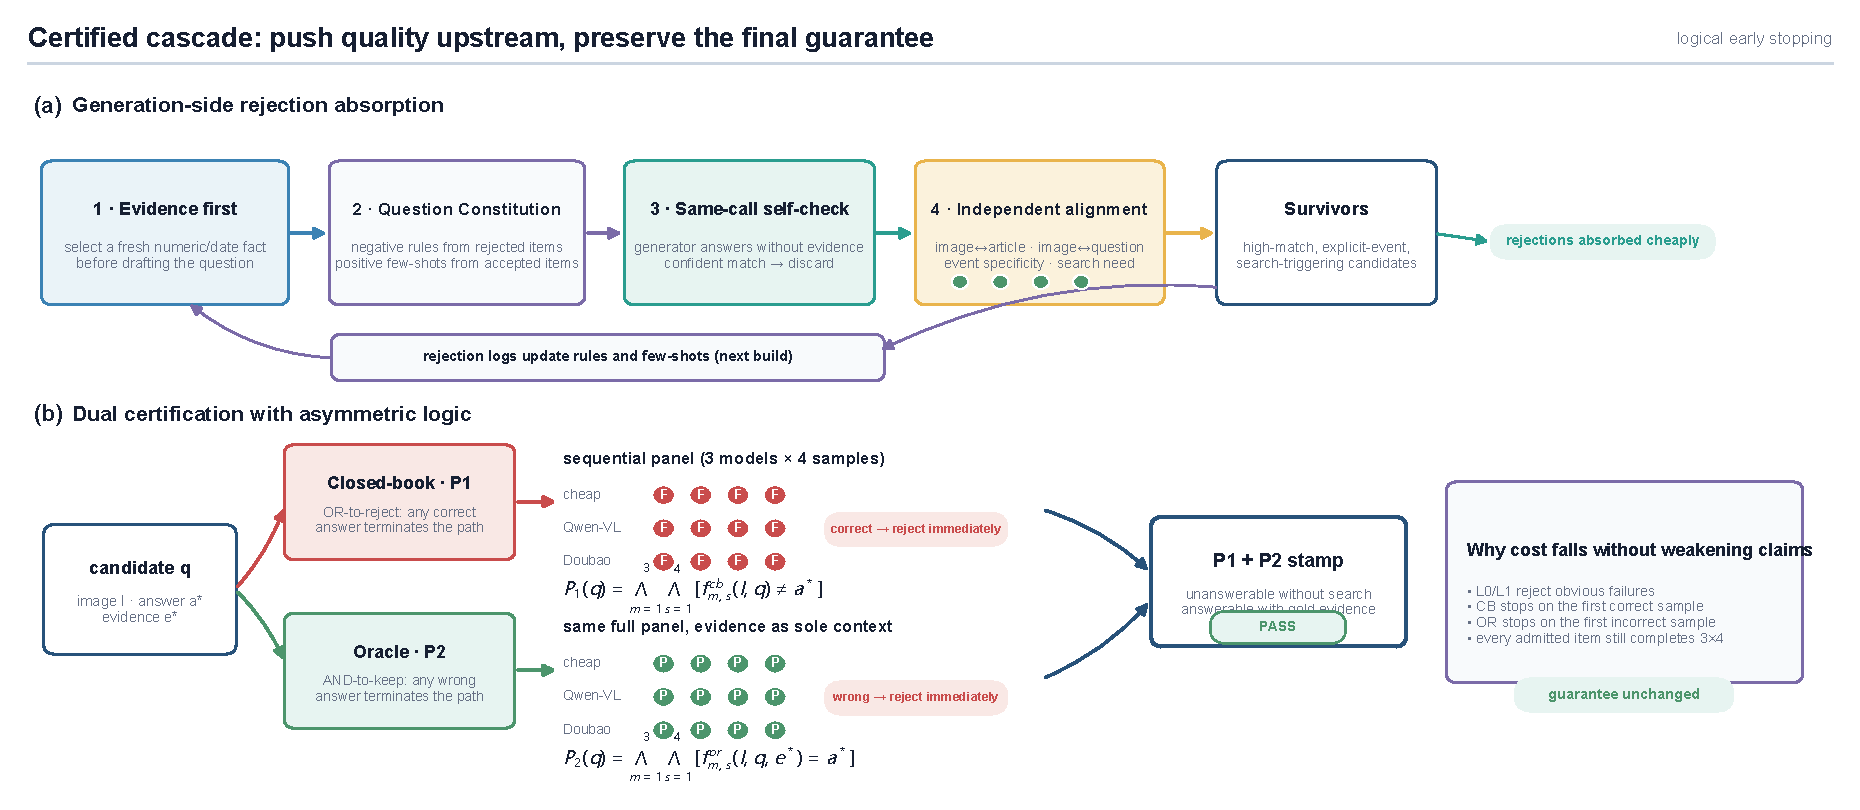
\includegraphics[width=\linewidth]{figures/fig2_certification_cascade.pdf}
  \caption{\textbf{Cost-aware certification cascade.} Cheap construction-time
  screens reshape the proposal distribution. Logical early stopping saves
  work only for rejected candidates; every admitted item retains the complete
  $3$-model $\times$ $4$-sample P1/P2 certificate.}
  \label{fig:cascade}
\end{figure}

\subsection{Why the two modules are trustworthy together}
The central trust argument is a separation of incentives, labels, and
evidence.
The generator is rewarded for producing many plausible candidates; the
quality module is rewarded for rejecting any candidate that violates the
contract.
Four design choices prevent this from becoming circular:
(i) exact source spans are checked against crawled text rather than accepted
from the generator;
(ii) two model families participate in the final panel;
(iii) universal quantification across models and samples makes admission
strict, while early stopping changes only compute;
and (iv) audit traces make every decision inspectable and re-certifiable.
Formally, admission is the conjunction
$P0(x)\land\neg\mathrm{Reject}_{\mathrm{CB}}(x)\land
\mathrm{Accept}_{\mathrm{OR}}(x)$; generator confidence is never an input to
this decision.
Human audit and cross-generator/panel-swap experiments in
Section~\ref{sec:experiments} test the residual risks rather than asking the
reader to trust model self-evaluation.

\section{Diagnostic Evaluation}
\label{sec:protocol}
Each agent is run on the same item in three conditions:
\begin{itemize}[leftmargin=*,itemsep=2pt]
  \item \textbf{Closed-book (CB):} image and question only;
  \item \textbf{With-search (WS):} the agent may issue web queries and open
  pages under a fixed tool budget;
  \item \textbf{Oracle (OR):} image, question, and gold evidence only.
\end{itemize}

We report exact/normalized short-answer accuracy and the search realization
ratio
\begin{equation}
\rho=\frac{\aws-\acb}{\aor-\acb},
\end{equation}
the fraction of certified answerable headroom realized by the agent's own
search.
For each WS error, fuzzy span matching and an adjudicator compare retrieved
documents to $e$.
Gold evidence absent implies a retrieval miss; gold present but unused
implies utilization failure; selecting a conflicting non-gold passage implies
distraction.

\begin{figure}[t]
  \centering
  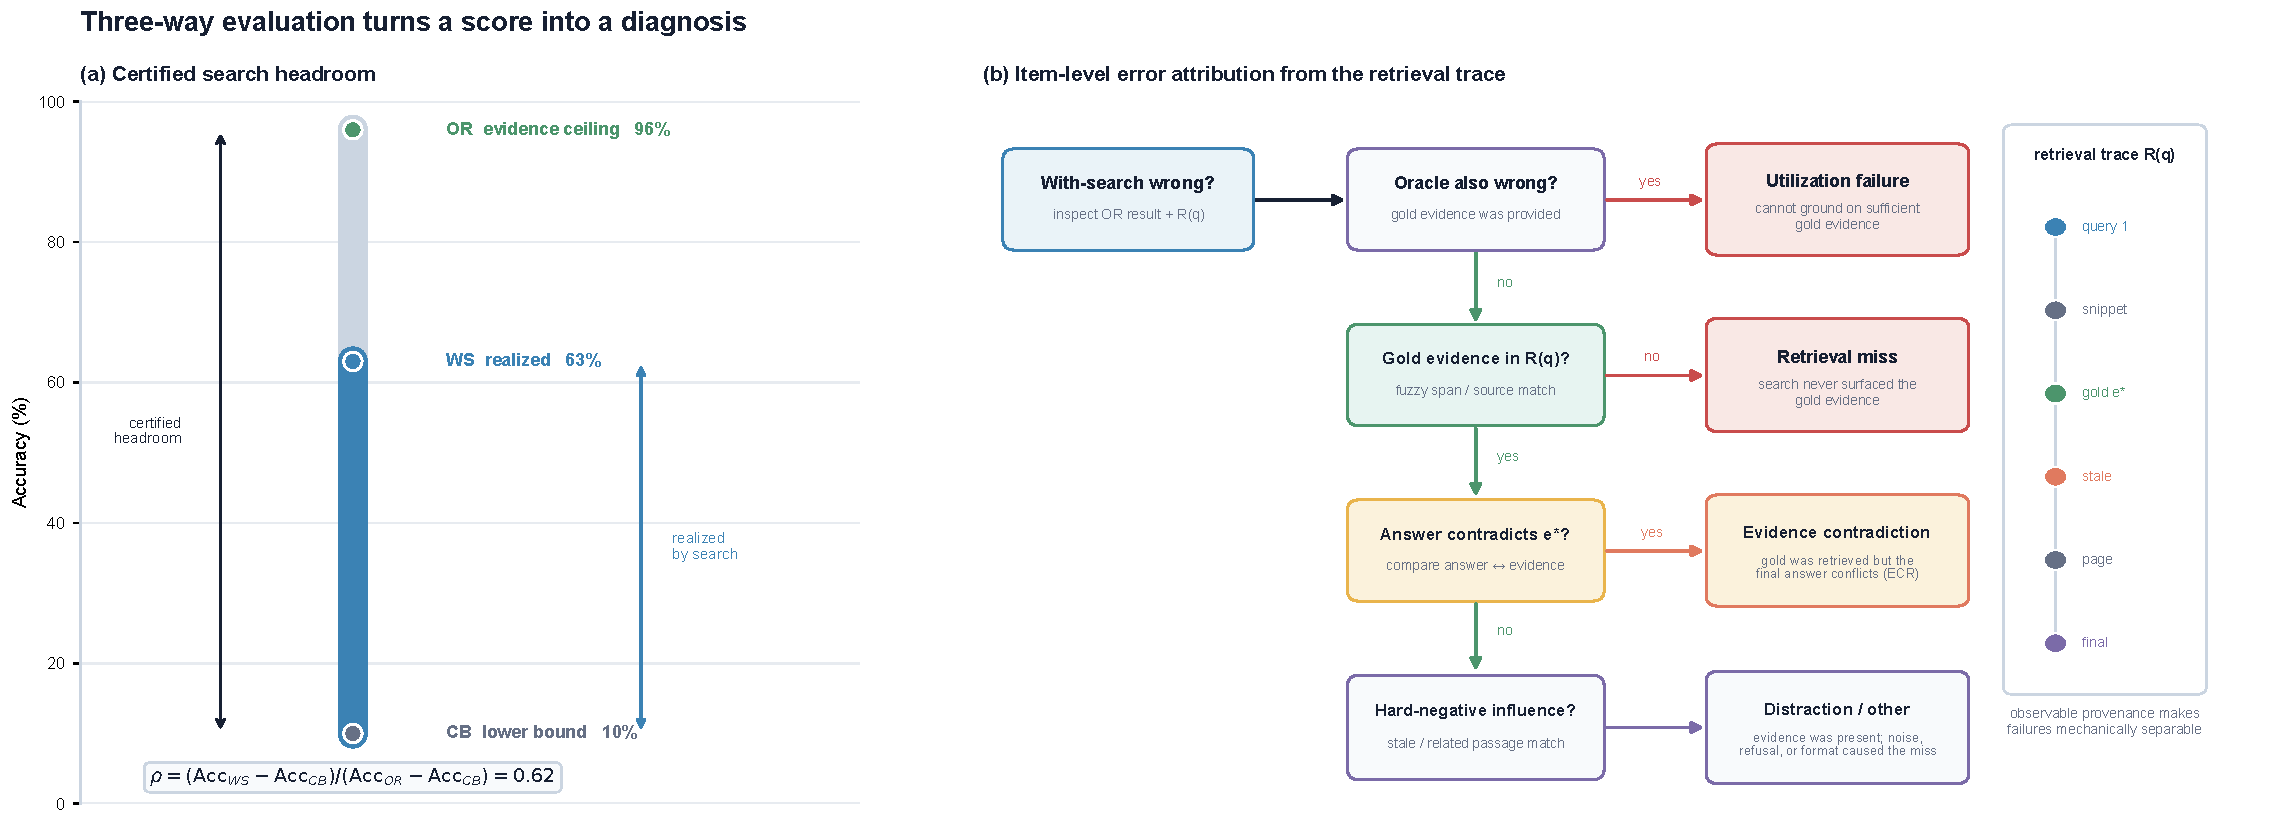
\includegraphics[width=\linewidth]{figures/fig3_diagnostic_protocol.pdf}
  \caption{\textbf{Three-way diagnostic.} P1 and P2 establish item-level
  endpoints. The WS trace then localizes failure to retrieval, distraction,
  or utilization instead of assigning every error to the model as a whole.}
  \label{fig:diagnostic}
\end{figure}

\section{Current Build Audit}
\label{sec:audit}
Table~\ref{tab:audit} reports measurements from the public 2026-08-15 build,
not simulated experiment values.
All 200 items pass the offline validator with zero errors or warnings.
They use 200 unique images and questions, cover 23 English-language sources,
and preserve all 24 panel predictions per item.

\begin{table}[t]
\centering
\small
\begin{tabular}{lr}
\toprule
Measured build property & Value\\
\midrule
Released items / unique images & 200 / 200\\
English-source items & 200 (100\%)\\
Numeric / temporal items & 103 / 54\\
Quantitative share & 157 (78.5\%)\\
Source domains & 23\\
Categories (politics/culture/business/sports/scitech) &
36/41/27/40/56\\
Image--article match, minimum & 4/4\\
Question--image grounding, minimum & 2/4\\
Certification profile & 3 models $\times$ 4 samples $\times$ 2 conditions\\
Offline validation & PASS (0 errors, 0 warnings)\\
\bottomrule
\end{tabular}
\caption{\textbf{Real current-build audit.} These values are computed from
\texttt{benchmark\_v2.json} and its validation report.}
\label{tab:audit}
\end{table}

A five-expert review is the independent second half of Experiment~1.
The appendix currently contains a \draftnote{} result schema in which all
\placeholder{200/200} items pass majority review, overall acceptability is
\placeholder{97.1\%} across 1,000 item--expert judgments, and Fleiss' $\kappa$
is \placeholder{.84} (Appendix~\ref{app:human}).
These numbers are not treated as measured evidence until the anonymized rating
matrix and annotator instructions are archived with the release.

\section{Experiments}
\label{sec:experiments}

\paragraph{Draft status.}
All blue values, Figures~\ref{fig:results} and~\ref{fig:error-decomp}, and the
appendix funnel/cost/human/error tables are simulated placeholders used to fix
the paper's hypotheses, reporting schema, and analysis plan before the full
evaluation is complete.

\subsection{Six experiments, one causal argument}
The evaluation is ordered so that each experiment licenses the next claim.
\textbf{Experiment 1 (release validity)} asks whether the engine can produce a
complete 200-item build satisfying the machine contract and an independent
five-expert audit.
\textbf{Experiment 2 (agent diagnosis)} measures CB, WS, and OR performance,
then labels retrieval traces; it separates missing knowledge from search,
retrieval, and evidence-use failures.
\textbf{Experiment 3 (generation ablation)} removes evidence-first proposal,
self-check, or rejection memory to test whether L0 actually reshapes the
candidate distribution toward P1/P2 rather than merely producing fluent text.
\textbf{Experiment 4 (certification ablation)} removes panel diversity or
early stopping to test, respectively, certificate transfer and computational
equivalence to exhaustive filtering.
\textbf{Experiment 5 (visual necessity)} masks, swaps, or removes the image and
visual gate to test whether performance depends on resolving a visual referent
rather than on a decorative news photograph.
\textbf{Experiment 6 (efficiency and stability)} reports calls, dollars, human
agreement, and matched builds across dates to test whether the mechanism is
practical and whether its conclusions persist beyond one news cycle.
Together, Experiments 1--2 establish validity and the scientific phenomenon;
Experiments 3--5 identify why it occurs; Experiment 6 tests whether the result
is affordable, reproducible, and temporally stable.

\subsection{Agents and protocol}
The target study compares proprietary search-native agents and open-weight
VLMs under a unified ReAct scaffold, with identical search endpoints,
top-$10$ retrieval, at most eight tool calls, and a frozen page snapshot.
Primary evaluation uses one 200-item on-demand build; the final submission
will repeat it across multiple build dates and report bootstrap confidence
intervals and paired McNemar tests.

\subsection{Experiments 1--2: release validity and agent diagnosis}
\begin{table}[t]
\centering
\small
\setlength{\tabcolsep}{5pt}
\begin{tabular}{lrrrr}
\toprule
Agent & CB$\downarrow$ & WS$\uparrow$ & OR$\uparrow$ & $\rho\uparrow$\\
\midrule
Claude Opus 5 & \placeholder{14.5} & \placeholder{\textbf{77.0}} &
\placeholder{\textbf{99.0}} & \placeholder{\textbf{.740}}\\
GPT-5.5 & \placeholder{22.5} & \placeholder{68.0} &
\placeholder{98.0} & \placeholder{.603}\\
Gemini 3.1 Pro & \placeholder{10.0} & \placeholder{63.0} &
\placeholder{95.5} & \placeholder{.620}\\
Qwen3.7 Plus & \placeholder{12.0} & \placeholder{58.0} &
\placeholder{96.5} & \placeholder{.544}\\
GLM-5V Turbo & \placeholder{12.5} & \placeholder{56.0} &
\placeholder{97.5} & \placeholder{.512}\\
Qwen3.7 Flash & \placeholder{12.0} & \placeholder{53.5} &
\placeholder{96.5} & \placeholder{.491}\\
Qwen3-VL-32B & \placeholder{5.5} & \placeholder{42.5} &
\placeholder{95.0} & \placeholder{.413}\\
Qwen3-VL-235B & \placeholder{7.0} & \placeholder{40.0} &
\placeholder{96.5} & \placeholder{.369}\\
Llama-4 Maverick & \placeholder{5.0} & \placeholder{36.0} &
\placeholder{94.0} & \placeholder{.348}\\
Qwen3-VL-8B & \placeholder{4.5} & \placeholder{32.5} &
\placeholder{89.5} & \placeholder{.329}\\
Qwen3-VL-30B-A3B & \placeholder{4.0} & \placeholder{30.5} &
\placeholder{92.0} & \placeholder{.301}\\
Llama-4 Scout & \placeholder{5.5} & \placeholder{28.0} &
\placeholder{94.0} & \placeholder{.254}\\
\bottomrule
\end{tabular}
\caption{\textbf{Simulated placeholder main table} (accuracy in \%).
The intended finding is a uniformly high oracle ceiling but a large,
model-dependent retrieval gap. Replace with measured runs before submission.}
\label{tab:main}
\end{table}

\begin{figure}[t]
  \centering
  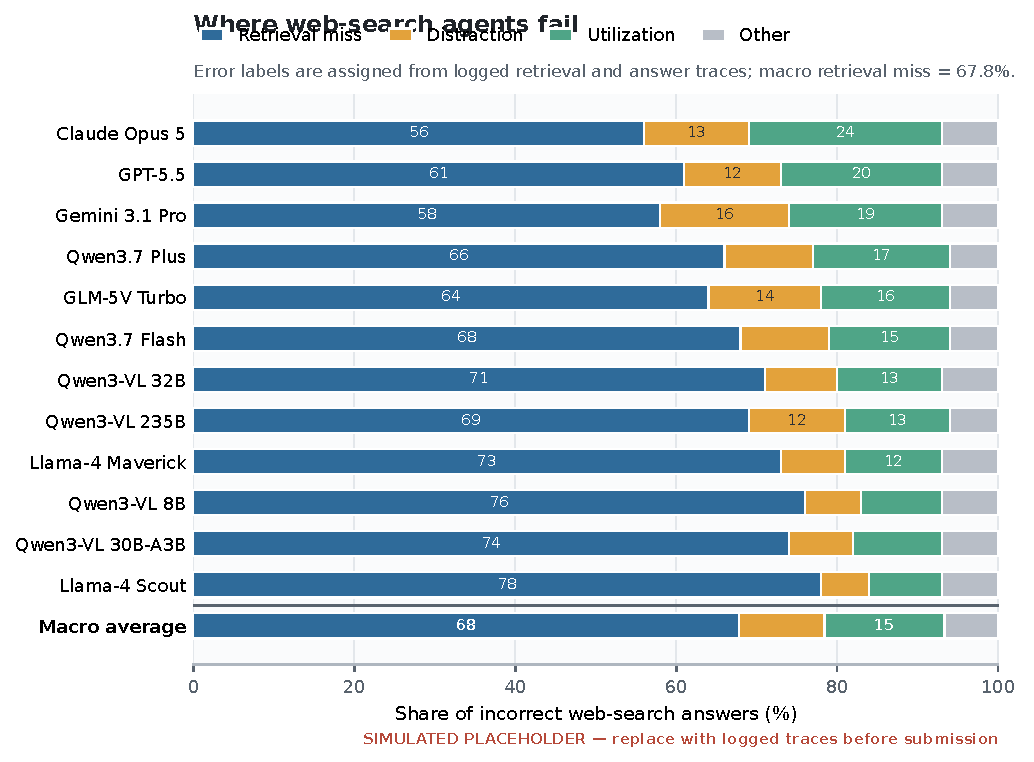
\includegraphics[width=\linewidth]{figures/fig5_error_decomposition.pdf}
  \caption{\textbf{Simulated placeholder error decomposition.} Each incorrect
  WS answer is labeled from the retrieval trace: \emph{retrieval miss} if no
  answer-bearing source is retrieved; \emph{distraction} if such a source is
  retrieved but a conflicting passage drives the answer; \emph{utilization}
  if the relevant evidence is retrieved but misread or not synthesized; and
  \emph{other} for tool failure or unclassifiable traces. The simulated macro
  share of retrieval misses is \placeholder{67.8\%}; this claim must be
  replaced by labels from logged runs before submission.}
  \label{fig:error-decomp}
\end{figure}

The intended headline is not that the best model scores
\placeholder{77.0\%}, but that it reaches only \placeholder{74.0\%} of its
own certified headroom.
High oracle scores across model families would validate P2 independently of
the construction panel, while large and heterogeneous OR--WS gaps would show
that the benchmark measures search rather than ordinary VQA.
The unchanged simulated pattern encodes three falsifiable predictions:
closed-book accuracy remains well below oracle accuracy, oracle performance
clusters near the ceiling, and with-search performance spreads widely across
agents.
Together these outcomes would show that items remain answerable while agent
rankings are driven primarily by search execution.
The scientific claim does not depend on which proprietary model wins; it
depends on the separation between the three conditions and on whether trace
labels explain the remaining gap.
An OR--WS gap alone cannot establish that retrieval is limiting: failure may
occur after relevant evidence was retrieved.
Accordingly, we make the stronger statement only if Figure~\ref{fig:error-decomp}
shows that retrieval-miss traces form the majority, with bootstrap intervals
over items, and if the held-out oracle remains near ceiling.
The simulated decomposition assigns \placeholder{67.8\%} of WS errors to
retrieval miss versus \placeholder{32.2\%} to all post-retrieval and other
causes combined; Appendix~\ref{app:errors} gives the operational labels and
worked traces.

\begin{figure}[t]
  \centering
  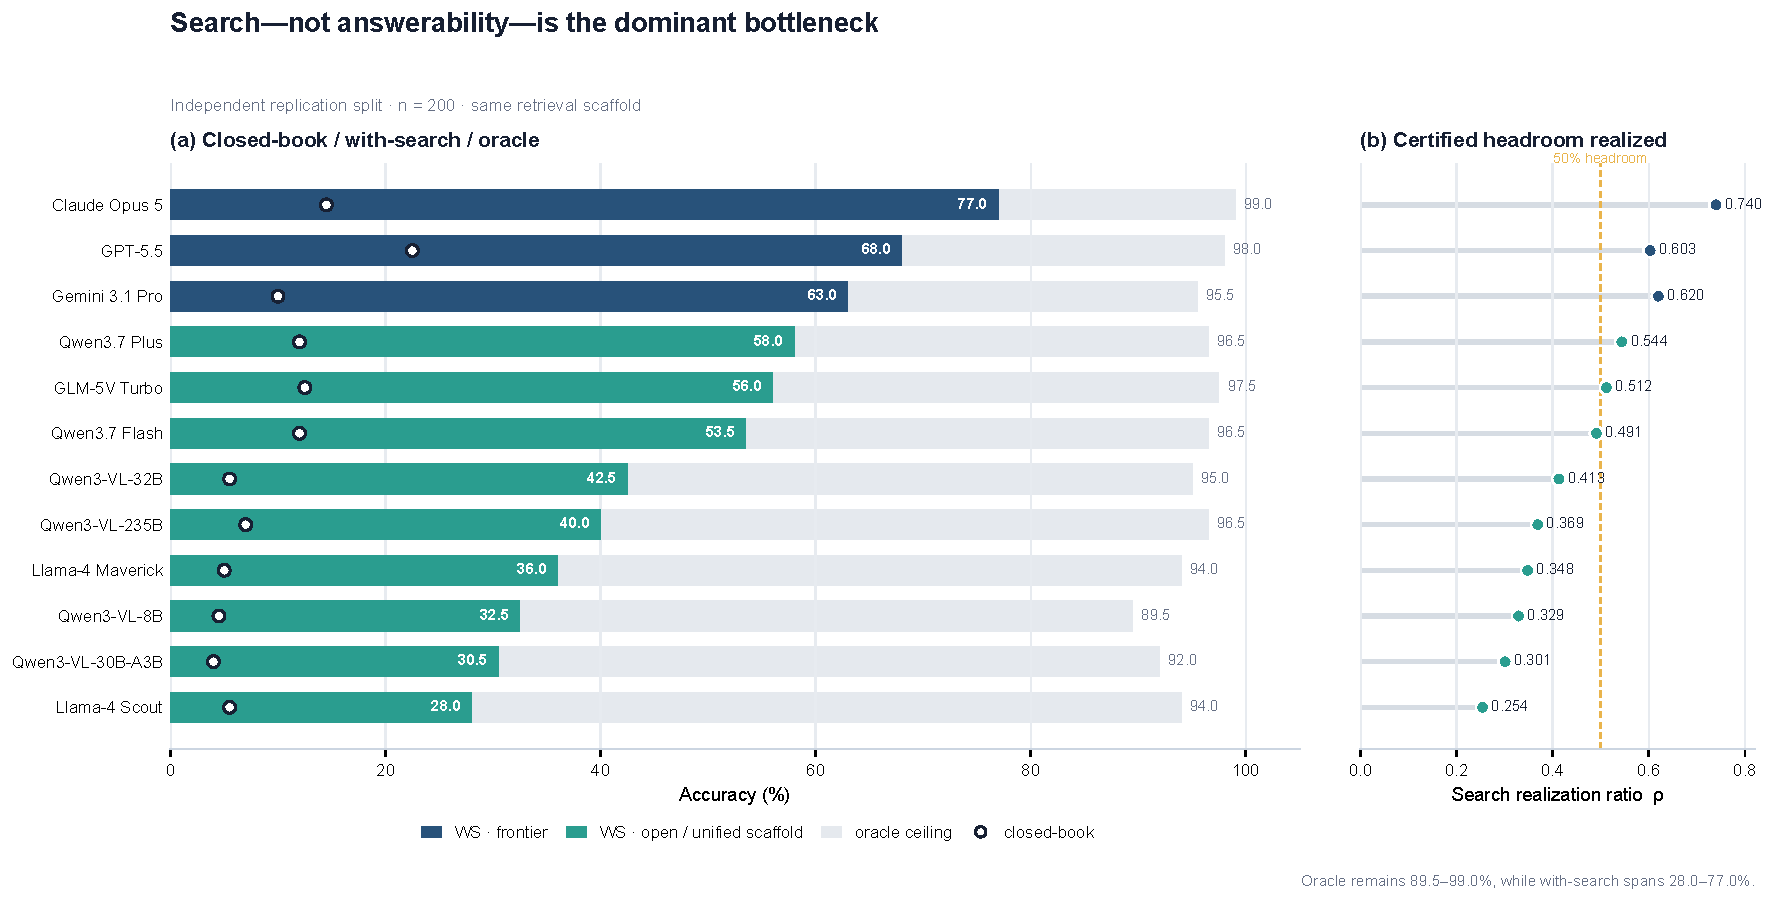
\includegraphics[width=\linewidth]{figures/fig4_main_results.pdf}
  \caption{\textbf{Simulated result visualization.} Draft values are retained
  to define the desired analysis and will be replaced with reproducible logs.}
  \label{fig:results}
\end{figure}

\subsection{Experiment 3: generation ablation}
We hold the article pool, images, quality module, and target size fixed and
compare four proposal policies: the full generator, question-first generation,
no same-call closed-book self-check, and no rejection-memory constitution.
The primary outcomes are P0/P1/P2 conditional yield and verified items per
1,000 generated candidates; secondary outcomes are evidence-span errors,
closed-book rejections, panel calls, and dollars per release.
This experiment is necessary because final validity alone cannot show whether
the proposed L0 design is useful: an arbitrarily wasteful generator could also
feed a strict verifier until 200 items survive.

\subsection{Experiment 4: certification ablation}
We compare a single judge, a same-family panel, and the heterogeneous
construction panel, then evaluate every admitted item with frozen held-out
model families.
The key transfer statistic is held-out CB leakage: the fraction of released
items that a model excluded from construction answers correctly without
search; we also report held-out oracle failure.
Thus ``P1 generalizes beyond the construction panel'' means only that held-out
models retain low CB accuracy---not that Equation~\ref{eq:p1} is a universal
proof.
A matched exhaustive run verifies that logical early stopping produces the
same accepted-set hash as all-at-once evaluation while reducing calls.

\subsection{Experiment 5: is the image really necessary?}
Four interventions distinguish visual grounding from decorative imagery:
(i) remove the image, (ii) mask the identity-bearing region, (iii) swap in a
same-topic image, and (iv) build without the visual gate.
Valid items should lose accuracy under removal/masking, fail predictably under
swaps, and preserve high oracle accuracy when the correct image is restored.
Humans additionally label whether the image resolves the omitted referent and
whether the question remains uniquely searchable without it.
This experiment is essential because high image--article similarity alone does
not establish causal image use.

\subsection{Experiment 6: efficiency, human validity, and time}
We report the complete construction funnel, calls, tokens, latency, and dollars
per accepted item for the cascade and exhaustive baseline.
Our preregistered draft expectation is approximately \placeholder{60\%} fewer
verification calls at an identical accepted-set hash, but this remains a
design estimate until a matched run is complete.
Five experts independently review all 200 items for answer correctness,
evidence sufficiency, image--article alignment, visual necessity, search
necessity, and overall acceptability; Appendix~\ref{app:human} gives the
annotation protocol and explicitly simulated table schema.
Finally, matched builds across dates report category mix, answer-type mix,
panel yield, agent ranking correlation, and metric variance.
A noise track injects same-day topical and stale look-alike passages to quantify
distraction separately from retrieval.

\section{Limitations and Validity}
P1 is empirical and panel-relative: a stronger future model may know an item
that the current panel does not.
On-demand re-certification and stored traces make this limitation measurable but
do not turn it into a universal theorem.
P2 establishes answerability from a clean evidence span, not robustness to
the noisy web.
News feeds introduce topical and geographic skew, and image licensing may
limit redistribution.
Finally, generator feedback can overfit to the verifier's blind spots; held-out
panels, cross-generator builds, and human audits are therefore part of the
main validity argument rather than optional appendix checks.

\section{Conclusion}
\bench{} treats live benchmark construction as a cooperative but asymmetric
generate--verify system.
Evidence-first generation and rejection-memory improve efficiency; strict,
auditable P0/P1/P2 certification establishes trust.
This separation lets us refresh on demand without weakening the central
claim, and turns the resulting benchmark from another visual QA score into a
diagnostic instrument for retrieval, distraction, and evidence use.

\subsubsection*{Reproducibility Statement}
Every released item stores its source span, timestamp, image provenance,
alignment scores, panel predictions, and certification trace.
The appendix specifies the release schema and thresholds; the final study will
release frozen retrieval snapshots, evaluation prompts, and paired agent logs.

\subsubsection*{Ethics and Data Use}
The benchmark uses public news sources and event imagery for research
evaluation.
The release preserves source attribution and URLs, avoids sensitive personal
inference, and documents image provenance; redistribution and long-term
archiving remain subject to source licensing and takedown requirements.

\subsubsection*{AI Use Statement}
Generative AI tools assisted with language editing, code prototyping, and
figure preparation.
The authors designed the method, review all source data and code, and remain
responsible for every scientific claim.
No AI-generated output is treated as empirical evidence without independent
validation, and all simulated values are explicitly marked in the draft.

\bibliographystyle{iclr2026_conference}
\bibliography{references}

\appendix
\section{Release Schema and Thresholds}
Each JSON record contains the question, short answer, answer type, exact
evidence, image path, source metadata, build date, visual anchor and event
fact, alignment audit, two referent-grounding audits, flattened panel
predictions, and the nested certification record.
The release validator requires:
(i) 200 items;
(ii) publication age within 48 hours;
(iii) exact evidence occurrence in the article;
(iv) every numeric answer token in the evidence;
(v) image--article score 4/4;
(vi) question--image score at least 2/4;
(vii) two consistent grounding samples;
and (viii) complete P1/P2 traces for all panel members.

\section{Answer-Equivalence Protocol}
\label{app:eq}
Table~\ref{tab:eq-examples} makes the grading boundary concrete.
The current fast path applies the normalizer described in
Section~\ref{sec:method}, accepts normalized equality, rejects unequal numeric
token sets, and accepts long normalized containment only when numeric tokens
agree.
All remaining cases go to a temperature-zero semantic judge; the primary
judge and provider-diverse fallback receive no evidence, retrieval trace,
candidate stage, or model identity.
The final release manifest will record whether a decision came from
\texttt{normalized-exact}, \texttt{numeric-reject},
\texttt{containment}, or \texttt{semantic-judge}.

\begin{table}[h]
\centering
\small
\setlength{\tabcolsep}{4pt}
\begin{tabular}{p{.23\linewidth}p{.23\linewidth}p{.13\linewidth}p{.31\linewidth}}
\toprule
Gold & Prediction & Verdict & Reason\\
\midrule
\$1.2 billion & 1.2 billion & correct & currency punctuation normalized\\
1.2 billion & 1.2 million & incorrect & scale changes the value\\
May 28, 2027 & 28 May 2027 & correct & same day after semantic check\\
May 2027 & May 28, 2027 & incorrect & date granularity differs\\
New York City & NYC & correct & entity alias after semantic check\\
12 km & 12 miles & incorrect & unit differs\\
\bottomrule
\end{tabular}
\caption{Normative equivalence examples. No approximate numeric tolerance is
used; equivalent unit conversions must be exact and explicitly recognized.}
\label{tab:eq-examples}
\end{table}

\section{Construction Algorithm, Funnel, and Rejections}
\label{app:construction}

\refstepcounter{algorithm}\label{alg:construction}
\noindent\fbox{\begin{minipage}{.95\linewidth}
\textbf{Algorithm \thealgorithm: Certificate-preserving construction}
\begin{enumerate}[leftmargin=*,itemsep=1pt,topsep=4pt]
  \item Crawl timestamped English articles inside the freshness window;
  retain a fetchable lead/body image and deduplicate articles and images.
  \item Generate $(q,a,e)$ evidence-first. Reject candidates that fail the
  same-call self-check, output schema, event-specificity, or exact-span rules.
  \item Apply P0/L1 deterministic, image--article, question--image, and two
  omitted-referent audits. Never repair a failed candidate.
  \item Evaluate P1 in cheap-to-expensive order. If any model/sample answers
  correctly closed-book, assign $\mathsf{N}$ and stop; otherwise retain all 12
  failures as the P1 certificate.
  \item Evaluate P2. If any model/sample fails with gold evidence, assign
  $\mathsf{S}$ and stop; otherwise retain all 12 successes as the P2
  certificate.
  \item Apply L3 deduplication and composition rules. Continue until 200 items
  survive, validate the complete temporary build, then atomically promote it.
  \item Publish the items, source snapshot, prompts, predictions, stage log,
  run manifest, and aggregate call/cost report.
\end{enumerate}
\end{minipage}}

\begin{table}[h]
\centering
\small
\setlength{\tabcolsep}{4pt}
\begin{tabular}{lrrp{.37\linewidth}}
\toprule
Stage & Survivors & Conditional yield & Dominant terminal rejection\\
\midrule
Fresh articles & \placeholder{1,200} & --- & no usable/deduplicated image\\
Generated candidates & \placeholder{820} & \placeholder{68.3\%} & $\mathsf{G}$ format/self-check\\
P0/L1 pass & \placeholder{470} & \placeholder{57.3\%} & $\mathsf{F,V,E}$ freshness/grounding/evidence\\
P1 pass & \placeholder{285} & \placeholder{60.6\%} & $\mathsf{N}$ closed-book leakage\\
P2 pass & \placeholder{236} & \placeholder{82.8\%} & $\mathsf{S}$ oracle failure\\
Released & \placeholder{200} & \placeholder{84.7\%} & $\mathsf{D}$ duplicate/quota\\
\bottomrule
\end{tabular}
\caption{\textbf{Simulated construction funnel.} Counts illustrate the exact
table to export from the immutable run manifest; they are not measurements.}
\label{tab:funnel}
\end{table}

\begin{table}[h]
\centering
\small
\setlength{\tabcolsep}{4pt}
\begin{tabular}{lp{.28\linewidth}p{.55\linewidth}}
\toprule
Code & Meaning & Representative raw reasons\\
\midrule
$\mathsf{G}$ & Generation/format & parse or missing field, answer type/length,
question form/language, generator self-reject\\
$\mathsf{F}$ & Fresh-event specificity & historical/background question,
non-event cue, stable attribute, fresh fact not central\\
$\mathsf{V}$ & Visual grounding & image--article mismatch, image-only answer,
omitted referent not resolved or not necessary\\
$\mathsf{E}$ & Evidence/answer span & evidence not verbatim, answer number absent,
ambiguous or unsupported visual claim\\
$\mathsf{N}$ & Search necessity (P1) & self-check answerable, any construction-panel
closed-book success, closed-book API failure\\
$\mathsf{S}$ & Evidence sufficiency (P2) & any construction-panel oracle failure or
unresolved equivalence decision\\
$\mathsf{D}$ & Release composition & perceptual/question duplicate, language or
quantitative quota, category cap\\
\bottomrule
\end{tabular}
\caption{Typed rejection taxonomy. The public log retains both this stable
group and the implementation-level raw reason.}
\label{tab:taxonomy}
\end{table}

\begin{table}[h]
\centering
\small
\begin{tabular}{lrrr}
\toprule
Verifier & Calls/build & Calls/release & API cost/build\\
\midrule
Exhaustive panel & \placeholder{18,920} & \placeholder{94.6} & \placeholder{\$18.20}\\
Logical cascade & \placeholder{7,610} & \placeholder{38.1} & \placeholder{\$7.32}\\
Relative change & \placeholder{$-59.8\%$} & \placeholder{$-59.8\%$} & \placeholder{$-59.8\%$}\\
\bottomrule
\end{tabular}
\caption{\textbf{Simulated efficiency schema.} The implied cascade cost is
\placeholder{\$0.0366} per released item. Pricing, cached tokens, retries, and
failed requests must be exported per provider for the measured table.}
\label{tab:cost}
\end{table}

\section{Five-Expert Human Audit}
\label{app:human}
Five experts independently inspect all 200 released items while blinded to
generator confidence and panel decisions.
For each item they answer six binary questions: gold answer correctness,
evidence sufficiency, image--article alignment, whether the image resolves the
question's omitted referent, whether finding the answer requires current web
information, and overall acceptability.
An item passes only if at least three of five experts answer yes to every
dimension.
We report the full $200\times5$ rating matrix, per-dimension positive rate,
item-level majority pass, Fleiss' $\kappa$, and disagreement notes.

\begin{table}[h]
\centering
\small
\setlength{\tabcolsep}{4pt}
\begin{tabular}{lrr}
\toprule
Criterion & Positive judgments / 1,000 & Fleiss' $\kappa$\\
\midrule
Answer correctness & \placeholder{996 (99.6\%)} & \placeholder{.92}\\
Evidence sufficiency & \placeholder{994 (99.4\%)} & \placeholder{.90}\\
Image--article alignment & \placeholder{998 (99.8\%)} & \placeholder{.95}\\
Image resolves omitted referent & \placeholder{982 (98.2\%)} & \placeholder{.86}\\
Search necessity & \placeholder{975 (97.5\%)} & \placeholder{.83}\\
Overall acceptability & \placeholder{971 (97.1\%)} & \placeholder{.84}\\
\midrule
Items passing majority on every criterion & \placeholder{200 / 200} & ---\\
Items with unanimous overall acceptance & \placeholder{176 / 200} & ---\\
\bottomrule
\end{tabular}
\caption{\textbf{Simulated placeholder human audit.} These values demonstrate
the reporting format and must be replaced by the archived expert rating
matrix; they are not empirical evidence.}
\label{tab:human}
\end{table}

\section{Error-Trace Protocol and Worked Examples}
\label{app:errors}
For each incorrect WS answer, the trace adjudicator first determines whether
any retrieved document contains an answer-bearing span equivalent to the gold
evidence.
If not, the label is retrieval miss.
If supporting evidence is present but the response follows a retrieved,
conflicting span, the label is distraction.
If supporting evidence is present and no conflicting span explains the error,
the label is utilization.
Tool/API failures and unresolved cases are other.
Adjudicators see the frozen trace but not the agent name; a stratified sample is
double-labeled to report agreement.

\begin{table}[h]
\centering
\small
\setlength{\tabcolsep}{3.5pt}
\begin{tabular}{lp{.29\linewidth}p{.29\linewidth}p{.20\linewidth}}
\toprule
Case & Retrieval trace & Answer behavior & Label\\
\midrule
A & Top-10 contains only older event pages; no gold-equivalent span & Agent
copies the prior event's number & Retrieval miss\\
B & Gold span at rank 4; stale conflicting number at rank 1 & Agent cites the
rank-1 number & Distraction\\
C & Gold span at rank 2 contains the exact amount and unit & Agent returns a
nearby number from the same paragraph & Utilization\\
D & Search endpoint times out before a result page is opened & No grounded
answer is produced & Other\\
\bottomrule
\end{tabular}
\caption{Synthetic worked traces illustrating mutually exclusive operational
labels. These are examples, not observations from the benchmark run.}
\label{tab:trace-examples}
\end{table}

\begin{table}[h]
\centering
\scriptsize
\setlength{\tabcolsep}{4pt}
\begin{tabular}{lrrrr}
\toprule
Agent & Retrieval miss & Distraction & Utilization & Other\\
\midrule
Claude Opus 5 & \placeholder{56} & \placeholder{13} & \placeholder{24} & \placeholder{7}\\
GPT-5.5 & \placeholder{61} & \placeholder{12} & \placeholder{20} & \placeholder{7}\\
Gemini 3.1 Pro & \placeholder{58} & \placeholder{16} & \placeholder{19} & \placeholder{7}\\
Qwen3.7 Plus & \placeholder{66} & \placeholder{11} & \placeholder{17} & \placeholder{6}\\
GLM-5V Turbo & \placeholder{64} & \placeholder{14} & \placeholder{16} & \placeholder{6}\\
Qwen3.7 Flash & \placeholder{68} & \placeholder{11} & \placeholder{15} & \placeholder{6}\\
Qwen3-VL-32B & \placeholder{71} & \placeholder{9} & \placeholder{13} & \placeholder{7}\\
Qwen3-VL-235B & \placeholder{69} & \placeholder{12} & \placeholder{13} & \placeholder{6}\\
Llama-4 Maverick & \placeholder{73} & \placeholder{8} & \placeholder{12} & \placeholder{7}\\
Qwen3-VL-8B & \placeholder{76} & \placeholder{7} & \placeholder{10} & \placeholder{7}\\
Qwen3-VL-30B-A3B & \placeholder{74} & \placeholder{8} & \placeholder{11} & \placeholder{7}\\
Llama-4 Scout & \placeholder{78} & \placeholder{6} & \placeholder{9} & \placeholder{7}\\
\midrule
Macro average & \placeholder{67.8} & \placeholder{10.6} & \placeholder{14.9} & \placeholder{6.7}\\
\bottomrule
\end{tabular}
\caption{\textbf{Simulated error decomposition} (\% of incorrect WS items).
Rows sum to 100 up to rounding. Replace with logged trace labels and bootstrap
confidence intervals.}
\label{tab:error-full}
\end{table}

\section{Reviewer-Facing Trust Checklist}
\begin{enumerate}[leftmargin=*]
  \item Can every gold answer be traced to an exact source span? \textbf{Yes.}
  \item Is the image necessary to resolve the omitted referent? \textbf{Audited
  twice and stored.}
  \item Can the construction panel answer without search? \textbf{No, across
  all 12 recorded attempts.}
  \item Can the panel answer from gold evidence? \textbf{Yes, across all 12
  recorded attempts.}
  \item Does early stopping change the admitted set? \textbf{No; it terminates
  only after the logical decision is already fixed.}
  \item Can claims be independently checked? \textbf{Yes; prompts,
  predictions, evidence, timestamps, and validation reports are released.}
\end{enumerate}

\end{document}
